%!TEX root = ../chapter2.tex
% ******************************* Thesis Appendix A ****************************
\chapter{}

\begin{figure}[H]
 \centering
    \begin{minipage}{0.8\textwidth}
        \centering
        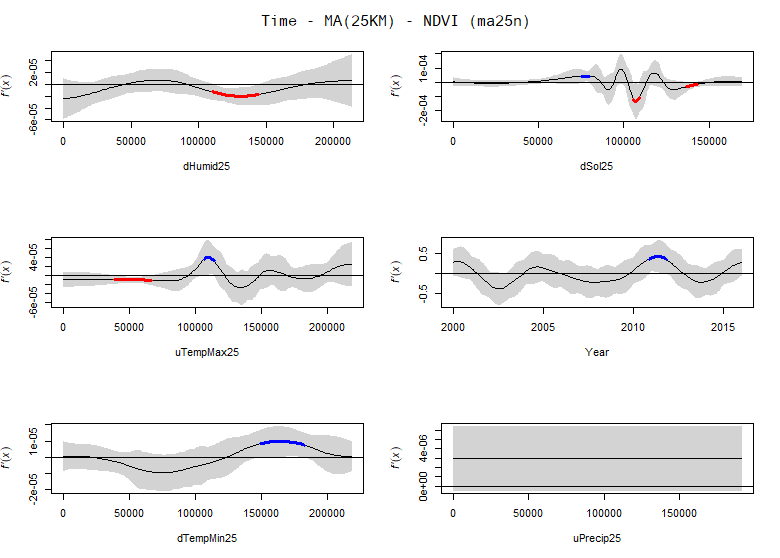
\includegraphics[width=1\textwidth]{ma25n.png} % first figure itself
        \caption{\textbf{Model ma25n}}
    \end{minipage}\hfill
    \begin{minipage}{0.8\textwidth}
        \centering
        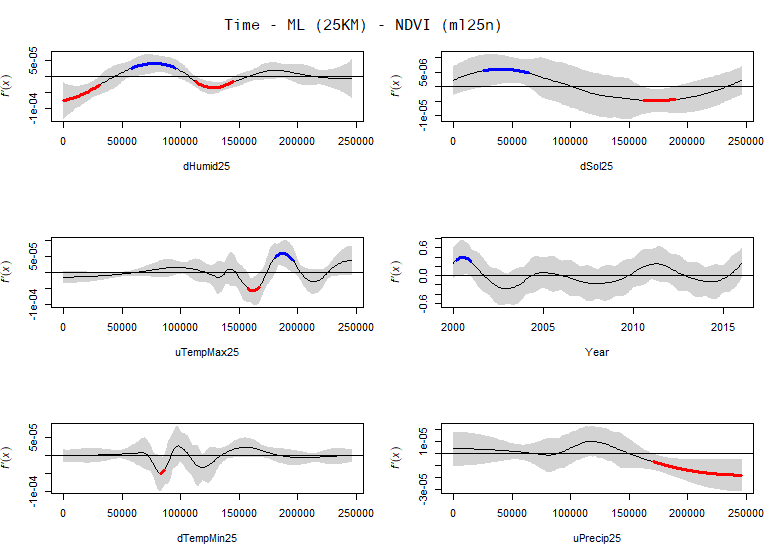
\includegraphics[width=1\textwidth]{ml25n.png} % second figure itself
        \caption{\textbf{Model ml25n}}
    \end{minipage}
\end{figure}

\begin{figure}[H]
 \centering
    \begin{minipage}{0.8\textwidth}
        \centering
        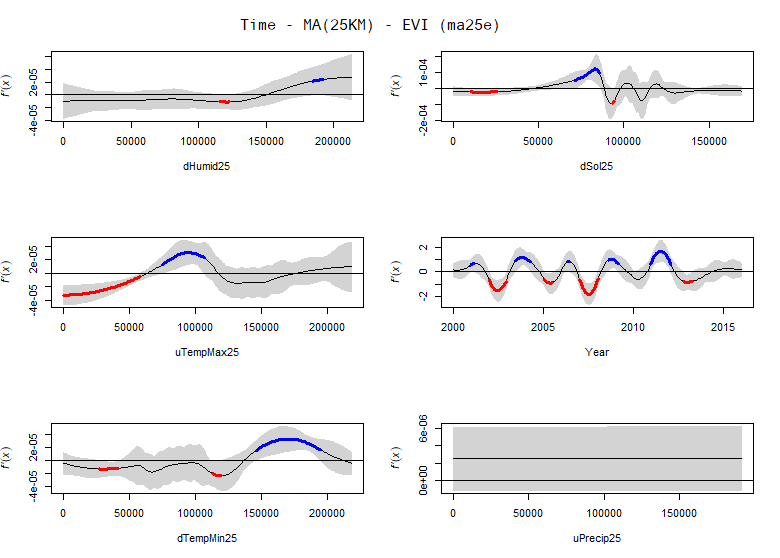
\includegraphics[width=1.2\textwidth]{ma25e.png} % first figure itself
        \caption{\textbf{Model ma25e}}
    \end{minipage}\hfill
    \begin{minipage}{0.8\textwidth}
        \centering
        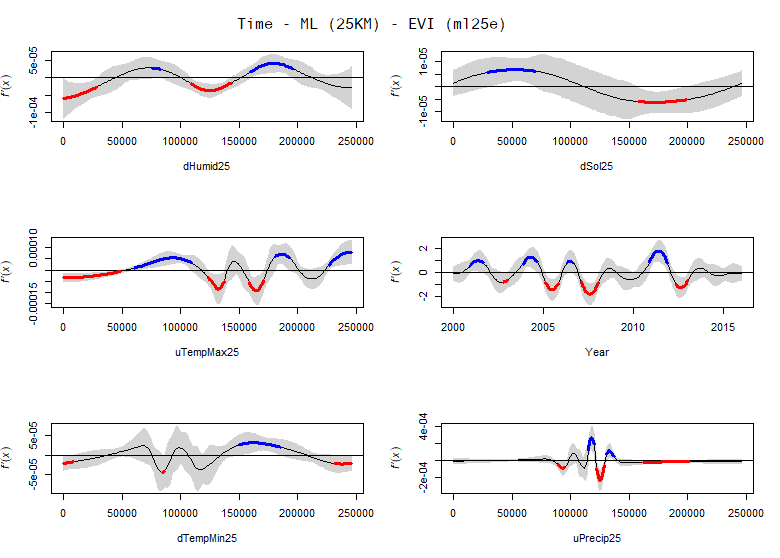
\includegraphics[width=1.2\textwidth]{ml25e.png} % second figure itself
        \caption{\textbf{Model ml25e}}
    \end{minipage}
\end{figure}

\begin{comment}
\begin{figure}[H]

    \begin{minipage}{0.8\textwidth}
        \centering
        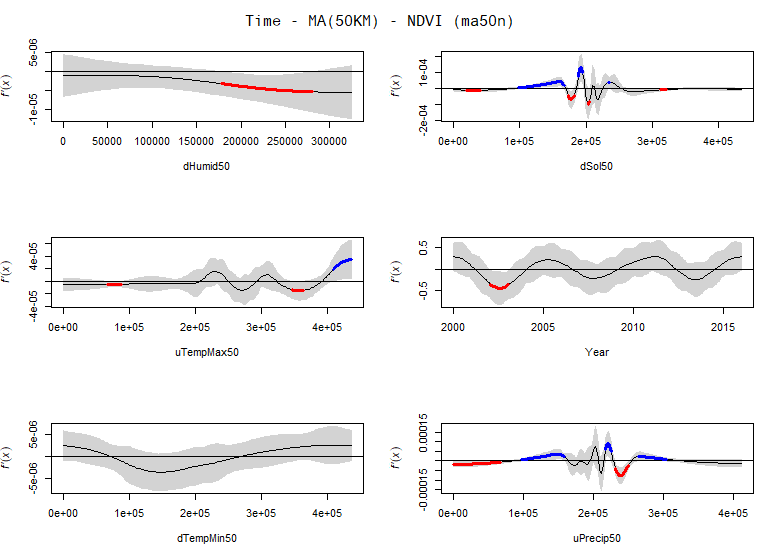
\includegraphics[width=1.2\textwidth]{ma50n.png} % first figure itself
        \caption{\textbf{Model ma50n}}
    \end{minipage}\hfill
    \begin{minipage}{0.8\textwidth}
        \centering
        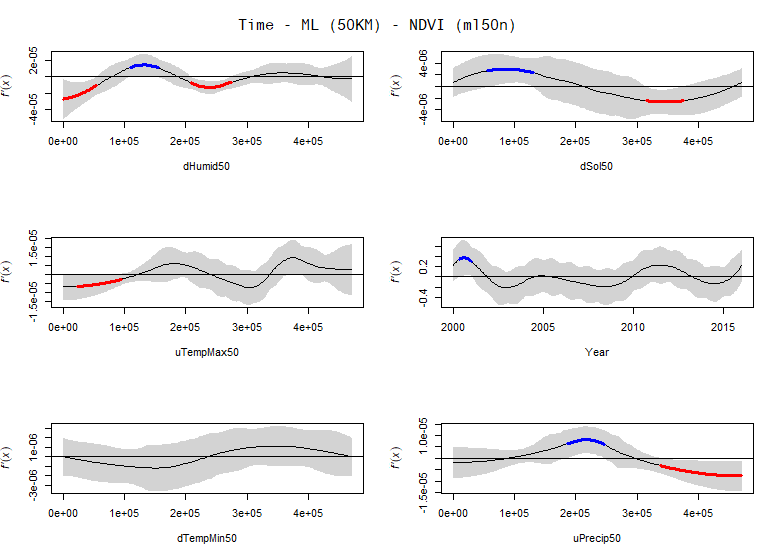
\includegraphics[width=1.2\textwidth]{ml50n.png} % second figure itself
        \caption{\textbf{Model ml50n}}
    \end{minipage}
\end{figure}

\begin{figure}[H]
 \centering
    \begin{minipage}{0.8\textwidth}
        \centering
        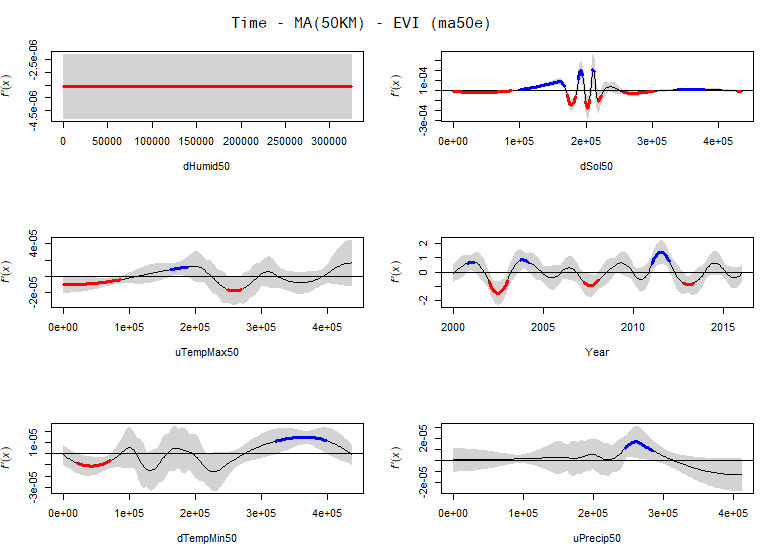
\includegraphics[width=1.2\textwidth]{ma50e.png} % first figure itself
        \caption{\textbf{Model ma50e}}
    \end{minipage}\hfill
    \begin{minipage}{0.8\textwidth}
        \centering
        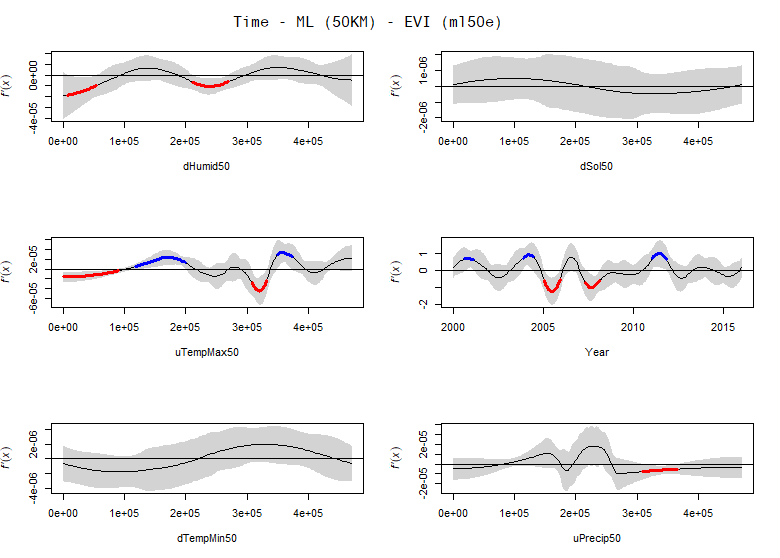
\includegraphics[width=1.2\textwidth]{ml50e.png} % second figure itself
        \caption{\textbf{Model ml50e}}
    \end{minipage}
\end{figure}

\begin{figure}[H]
    \begin{minipage}{0.8\textwidth}
        \centering
        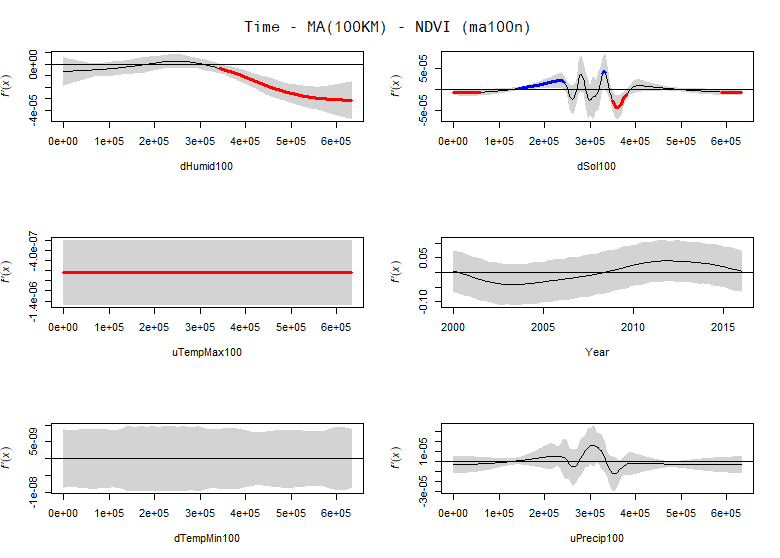
\includegraphics[width=1.2\textwidth]{ma100n.png} % first figure itself
        \caption{\textbf{Model ma100n}}
    \end{minipage}\hfill
    \begin{minipage}{0.8\textwidth}
        \centering
        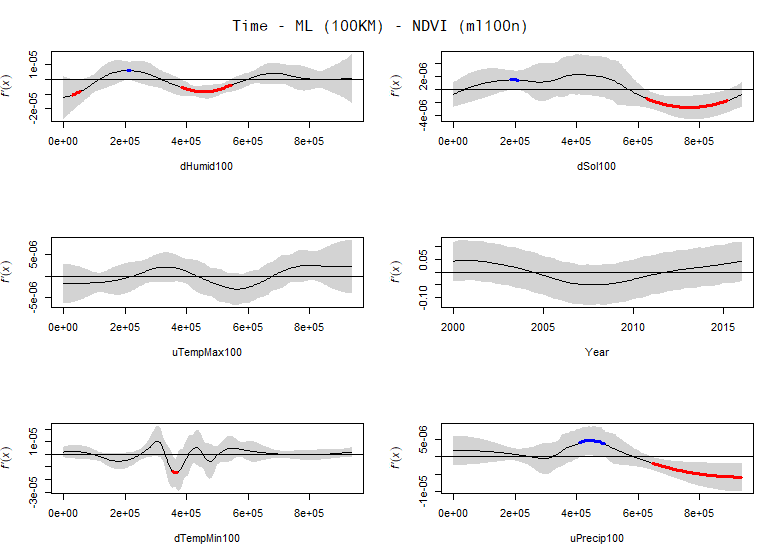
\includegraphics[width=1.2\textwidth]{ml100n.png} % second figure itself
        \caption{\textbf{Model ml100n}}
    \end{minipage}
\end{figure}

\begin{figure}[H]
 \centering
    \begin{minipage}{0.8\textwidth}
        \centering
        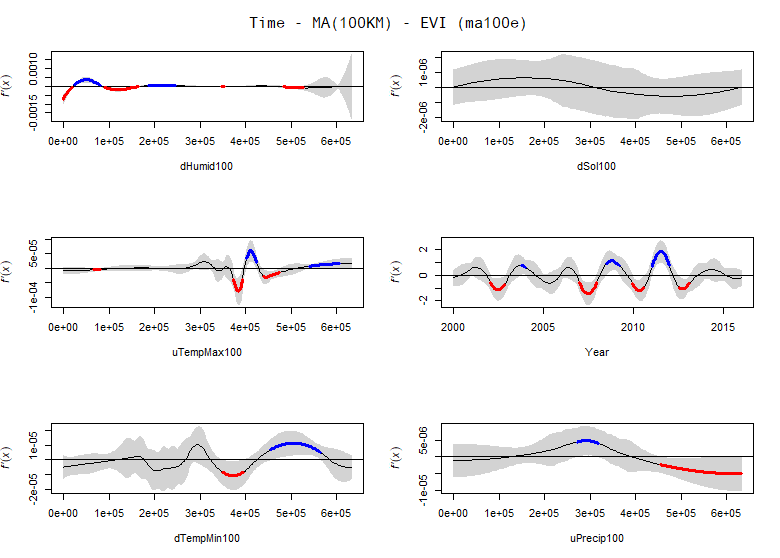
\includegraphics[width=1.2\textwidth]{ma100e.png} % first figure itself
        \caption{\textbf{Model ma100e}}
    \end{minipage}\hfill
    \begin{minipage}{0.8\textwidth}
        \centering
        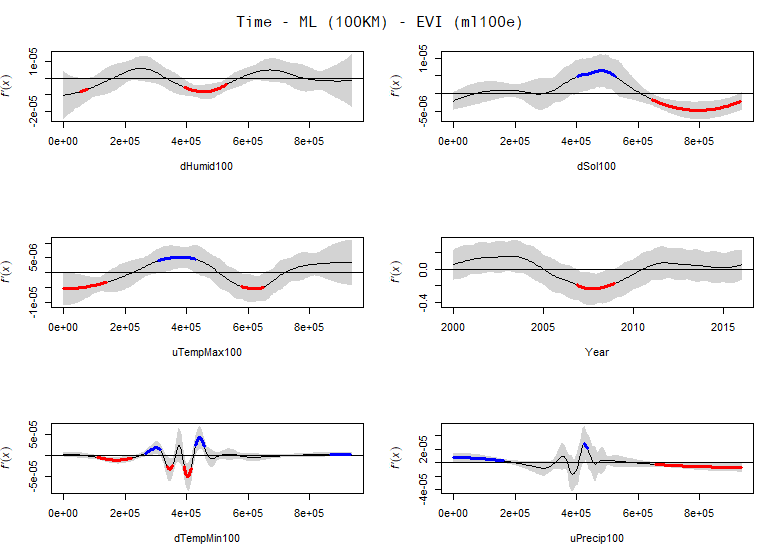
\includegraphics[width=1.2\textwidth]{ml100e.png} % second figure itself
        \caption{\textbf{Model ml100e}}
    \end{minipage}
\end{figure}
\end{comment}

\begin{figure}[H]
 \centering
    \begin{minipage}{0.8\textwidth}
        \centering
        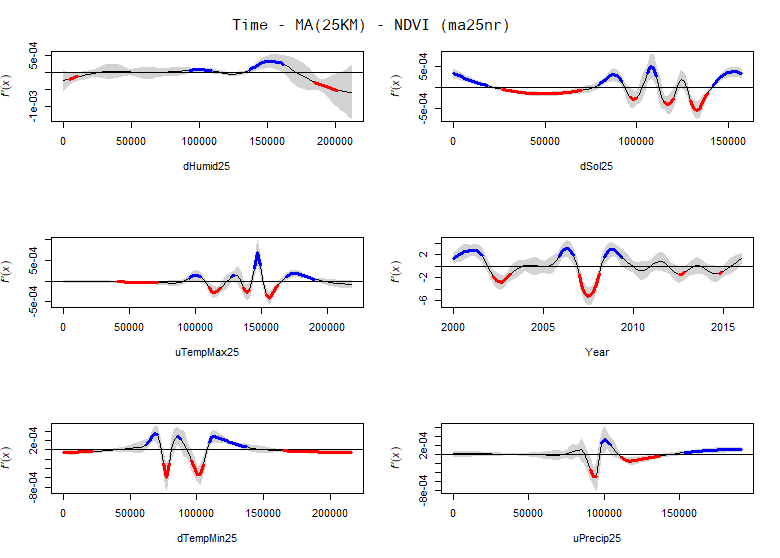
\includegraphics[width=1.2\textwidth]{ma25nr.png} % first figure itself
        \caption{\textbf{Model ma25nr}}
    \end{minipage}\hfill
    \begin{minipage}{0.8\textwidth}
        \centering
        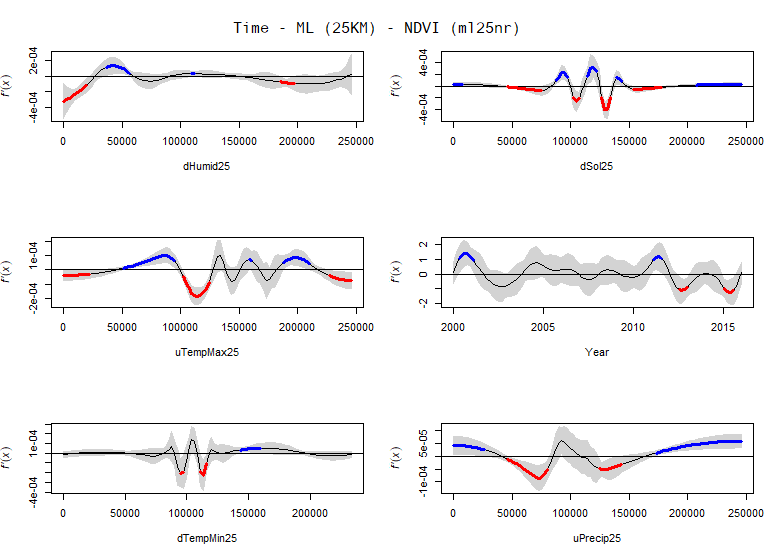
\includegraphics[width=1.2\textwidth]{ml25nr.png} % second figure itself
        \caption{\textbf{Model ml25nr}}
    \end{minipage}
\end{figure}

\begin{figure}[H]
 \centering
    \begin{minipage}{0.8\textwidth}
        \centering
        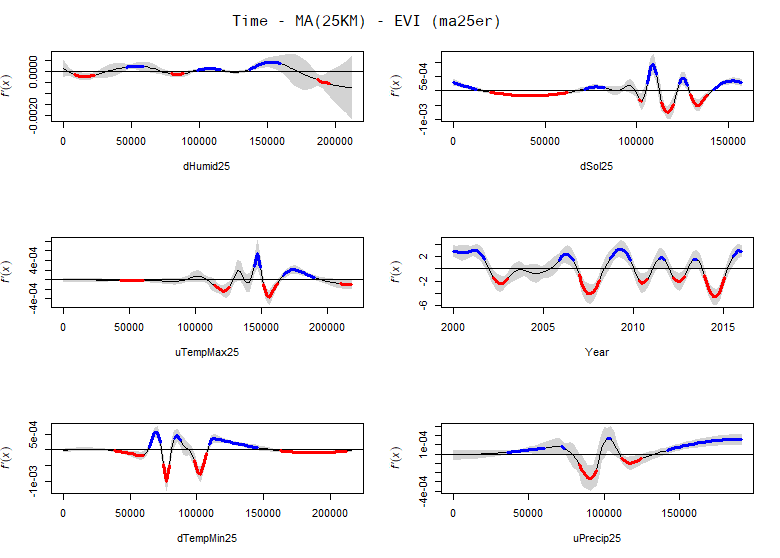
\includegraphics[width=1.2\textwidth]{ma25er.png} % first figure itself
        \caption{\textbf{Model ma25er}}
    \end{minipage}\hfill
    \begin{minipage}{0.8\textwidth}
        \centering
        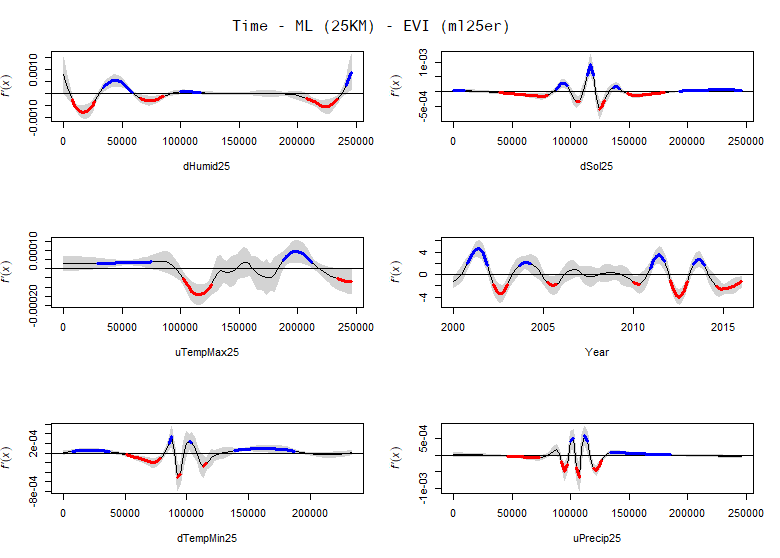
\includegraphics[width=1.2\textwidth]{ml25er.png} % second figure itself
        \caption{\textbf{Model ml25er}}
    \end{minipage}
\end{figure}

\begin{figure}[H]

    \begin{minipage}{0.8\textwidth}
        \centering
        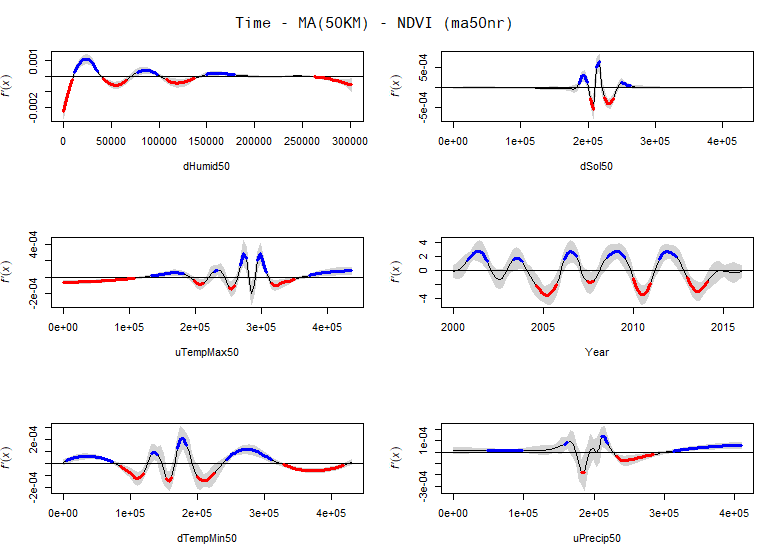
\includegraphics[width=1.2\textwidth]{ma50nr.png} % first figure itself
        \caption{\textbf{Model ma50nr}}
    \end{minipage}\hfill
    \begin{minipage}{0.8\textwidth}
        \centering
        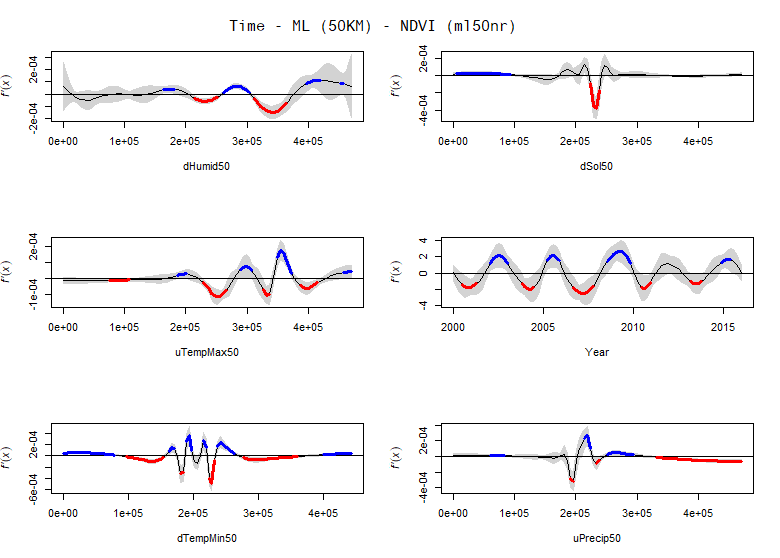
\includegraphics[width=1.2\textwidth]{ml50nr.png} % second figure itself
        \caption{\textbf{Model ml50nr}}
    \end{minipage}
\end{figure}

\begin{figure}[H]
 \centering
    \begin{minipage}{0.8\textwidth}
        \centering
        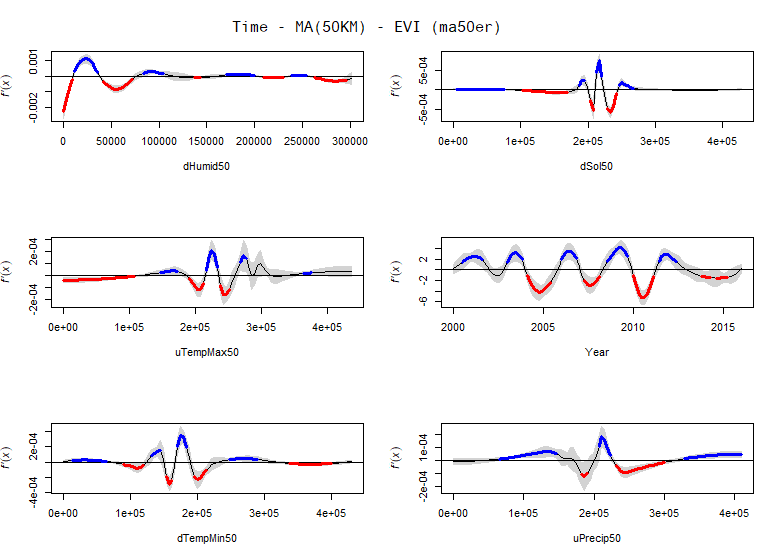
\includegraphics[width=1.2\textwidth]{ma50er.png} % first figure itself
        \caption{\textbf{Model ma50er}}
    \end{minipage}\hfill
    \begin{minipage}{0.8\textwidth}
        \centering
        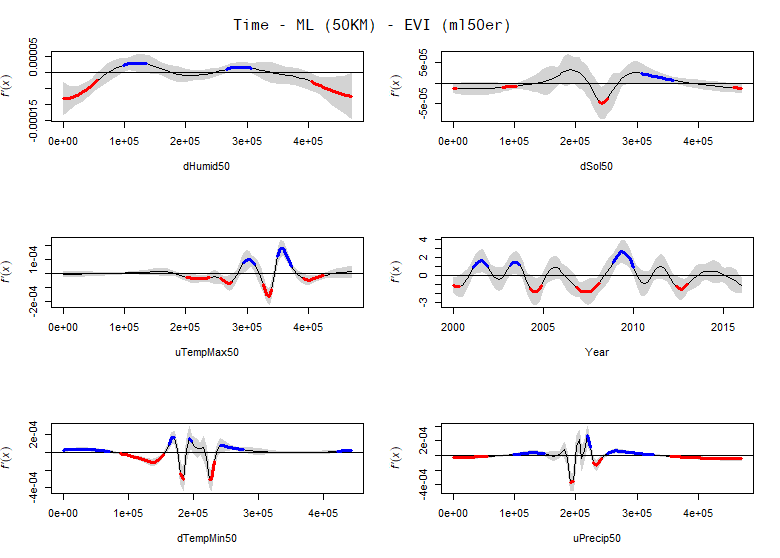
\includegraphics[width=1.2\textwidth]{ml50er.png} % second figure itself
        \caption{\textbf{Model ml50er}}
    \end{minipage}
\end{figure}

\begin{figure}[H]
    \begin{minipage}{0.8\textwidth}
        \centering
        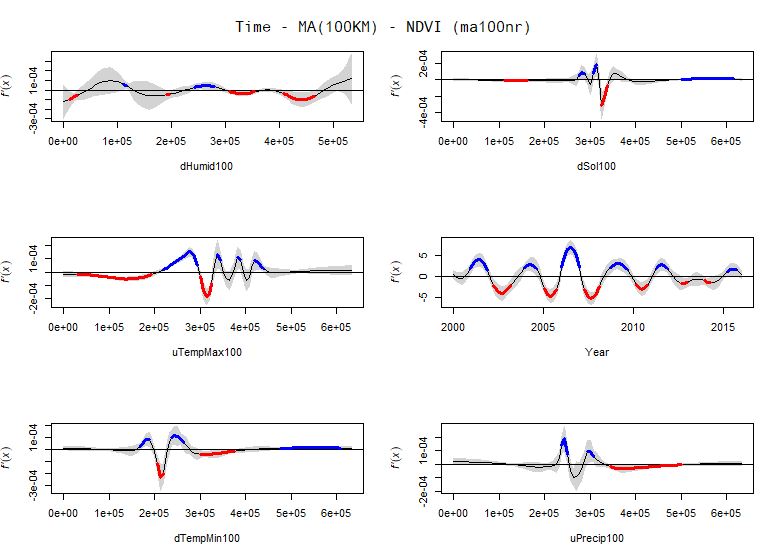
\includegraphics[width=1.2\textwidth]{ma100nr.png} % first figure itself
        \caption{\textbf{Model ma100nr}}
    \end{minipage}\hfill
    \begin{minipage}{0.8\textwidth}
        \centering
        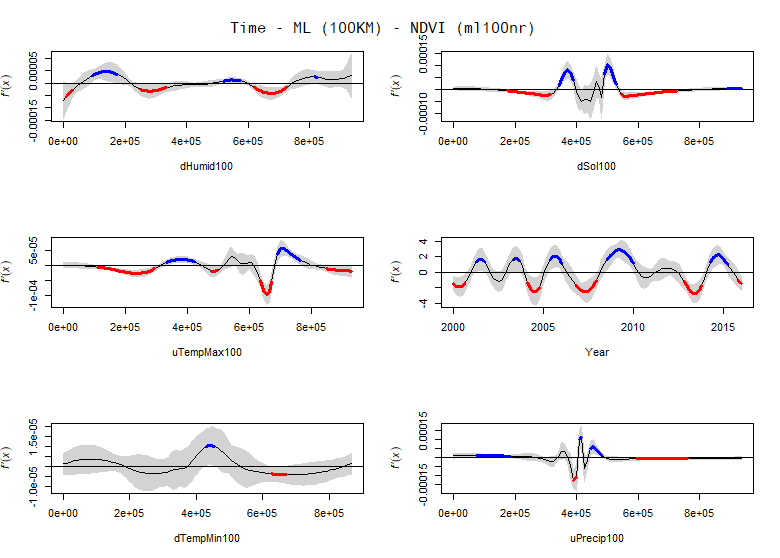
\includegraphics[width=1.2\textwidth]{ml100nr.png} % second figure itself
        \caption{\textbf{Model ml100nr}}
    \end{minipage}
\end{figure}

\begin{figure}[H]
 \centering
    \begin{minipage}{0.8\textwidth}
        \centering
        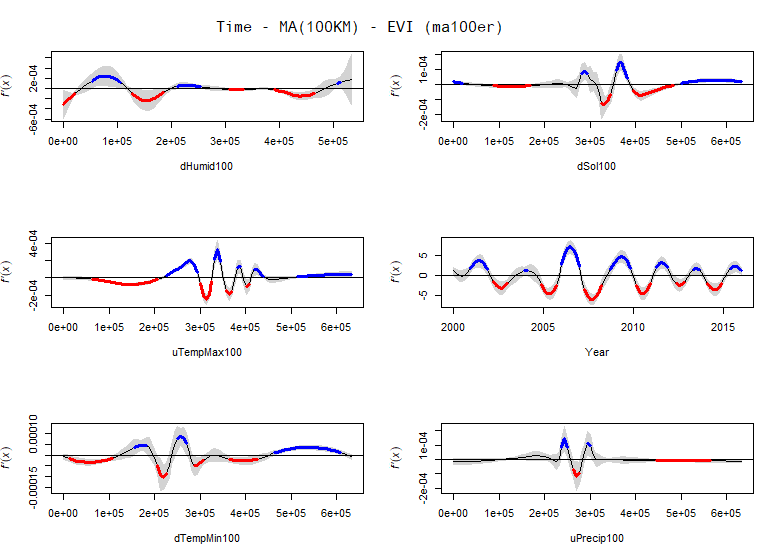
\includegraphics[width=1.2\textwidth]{ma100er.png} % first figure itself
        \caption{\textbf{Model ma100er}}
    \end{minipage}\hfill
    \begin{minipage}{0.8\textwidth}
        \centering
        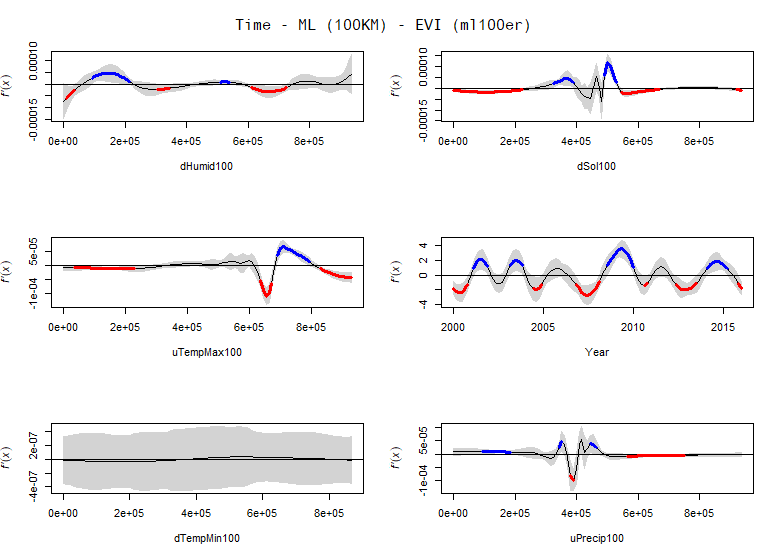
\includegraphics[width=1.2\textwidth]{ml100er.png} % second figure itself
        \caption{\textbf{Model ml100er}}
    \end{minipage}
\end{figure}

\begin{figure}[H]
 \centering
    \begin{minipage}{0.8\textwidth}
        \centering
        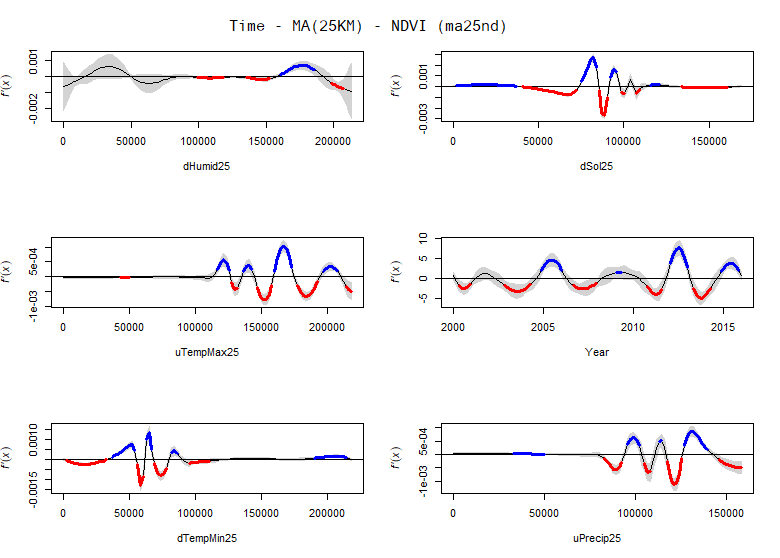
\includegraphics[width=1.2\textwidth]{ma25nd.png} % first figure itself
        \caption{\textbf{Model ma25nd}}
    \end{minipage}\hfill
    \begin{minipage}{0.8\textwidth}
        \centering
        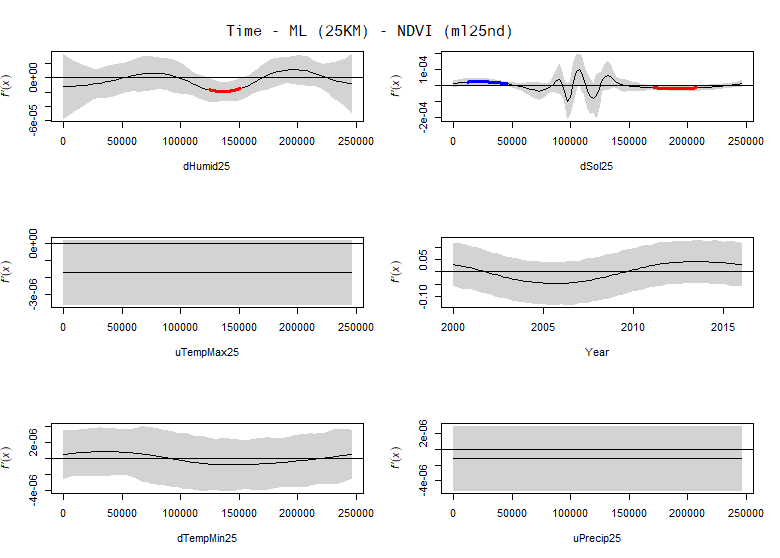
\includegraphics[width=1.2\textwidth]{ml25nd.png} % second figure itself
        \caption{\textbf{Model ml25nd}}
    \end{minipage}
\end{figure}

\begin{figure}[H]
 \centering
    \begin{minipage}{0.8\textwidth}
        \centering
        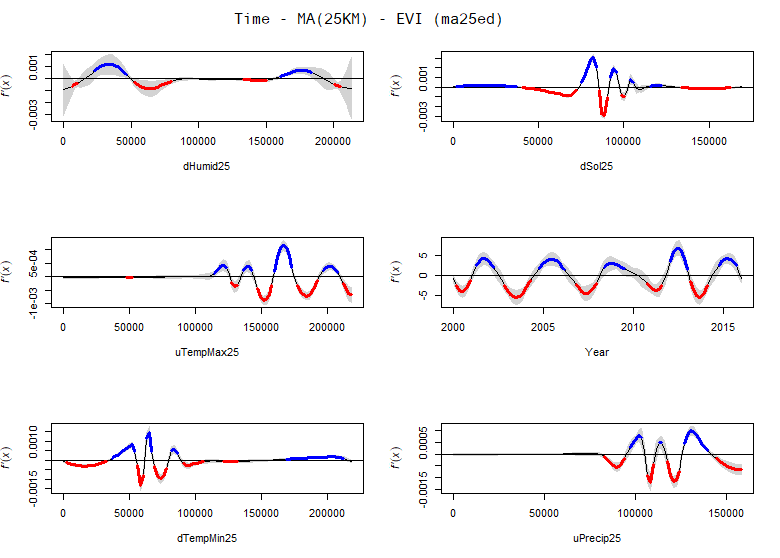
\includegraphics[width=1.2\textwidth]{ma25ed.png} % first figure itself
        \caption{\textbf{Model ma25ed}}
    \end{minipage}\hfill
    \begin{minipage}{0.8\textwidth}
        \centering
        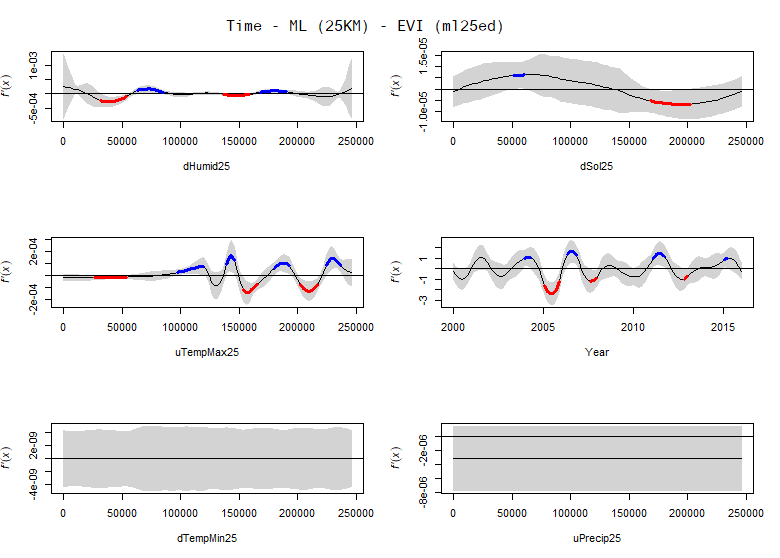
\includegraphics[width=1.2\textwidth]{ml25ed.png} % second figure itself
        \caption{\textbf{Model ml25ed}}
    \end{minipage}
\end{figure}

\begin{figure}[H]

    \begin{minipage}{0.8\textwidth}
        \centering
        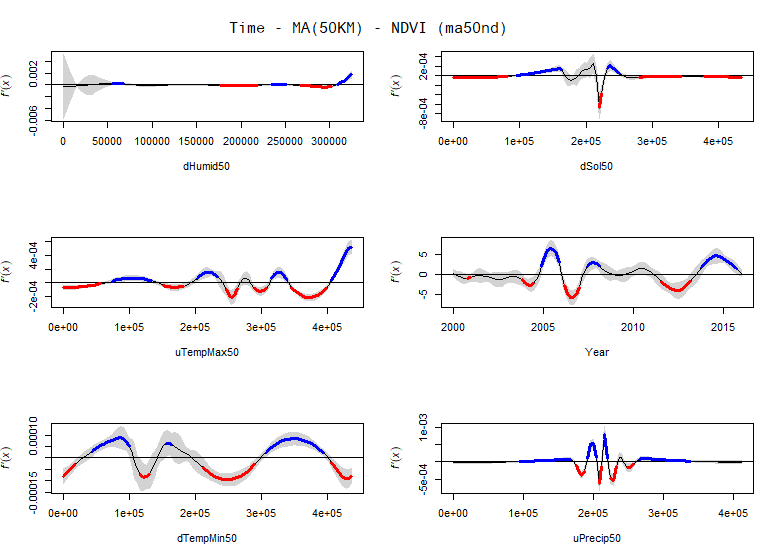
\includegraphics[width=1.2\textwidth]{ma50nd.png} % first figure itself
        \caption{\textbf{Model ma50nd}}
    \end{minipage}\hfill
    \begin{minipage}{0.8\textwidth}
        \centering
        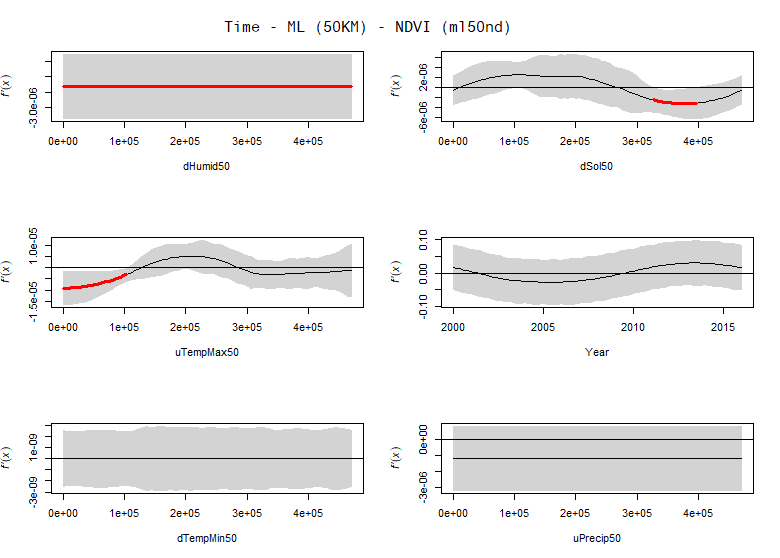
\includegraphics[width=1.2\textwidth]{ml50nd.png} % second figure itself
        \caption{\textbf{Model ml50nd}}
    \end{minipage}
\end{figure}

\begin{figure}[H]
 \centering
    \begin{minipage}{0.8\textwidth}
        \centering
        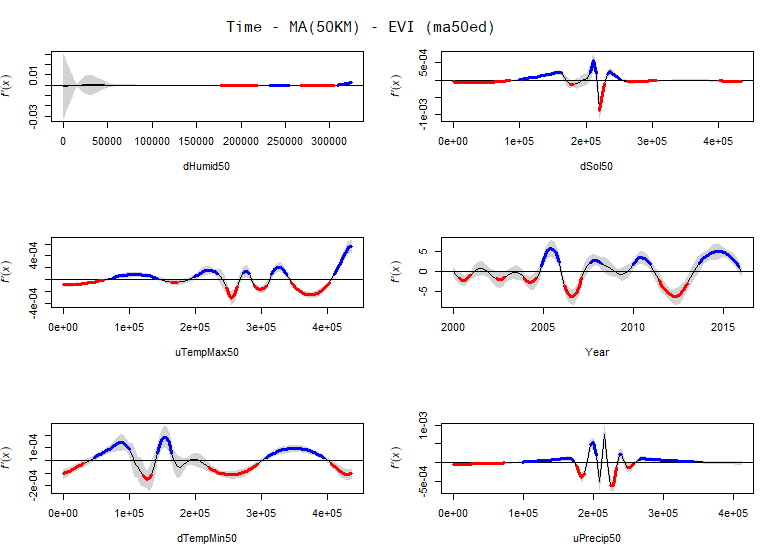
\includegraphics[width=1.2\textwidth]{ma50ed.png} % first figure itself
        \caption{\textbf{Model ma50ed}}
    \end{minipage}\hfill
    \begin{minipage}{0.8\textwidth}
        \centering
        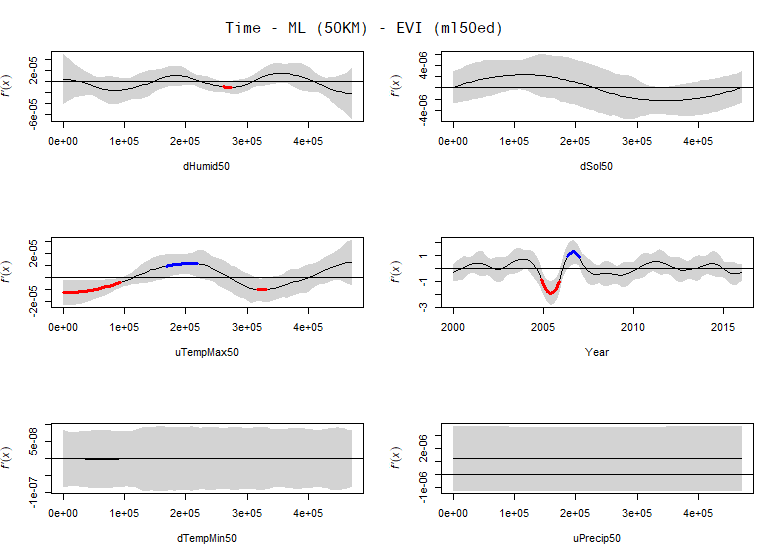
\includegraphics[width=1.2\textwidth]{ml50ed.png} % second figure itself
        \caption{\textbf{Model ml50ed}}
    \end{minipage}
\end{figure}

\begin{figure}[H]
    \begin{minipage}{0.8\textwidth}
        \centering
        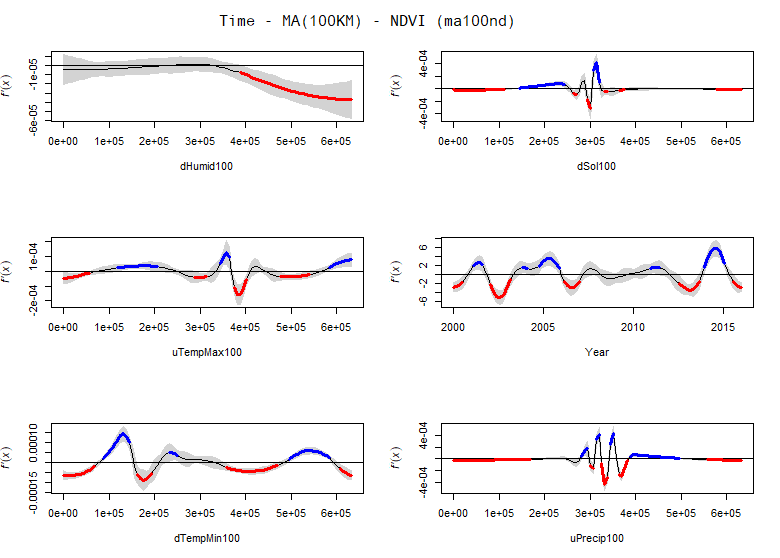
\includegraphics[width=1.2\textwidth]{ma100nd.png} % first figure itself
        \caption{\textbf{Model ma100nd}}
    \end{minipage}\hfill
    \begin{minipage}{0.8\textwidth}
        \centering
        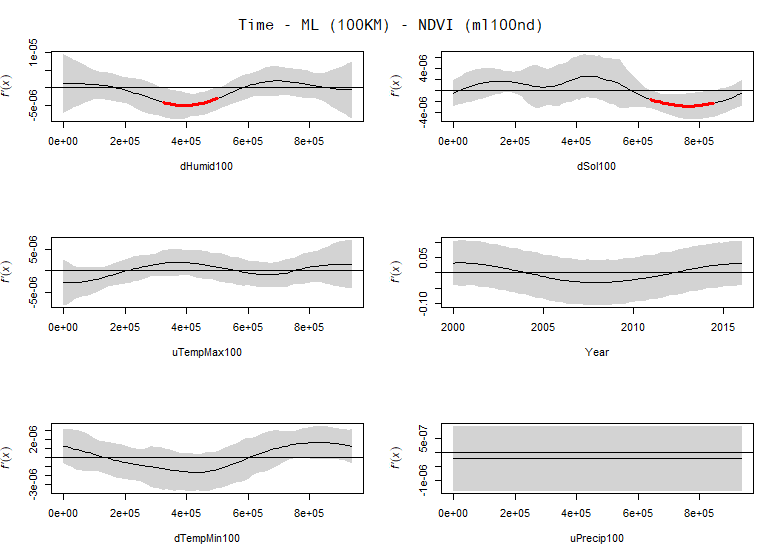
\includegraphics[width=1.2\textwidth]{ml100nd.png} % second figure itself
        \caption{\textbf{Model ml100nd}}
    \end{minipage}
\end{figure}

\begin{figure}[H]
 \centering
    \begin{minipage}{0.8\textwidth}
        \centering
        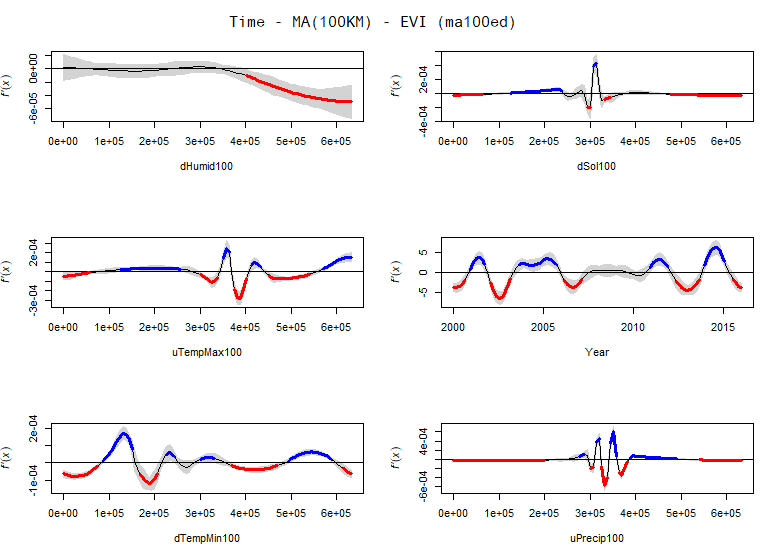
\includegraphics[width=1.2\textwidth]{ma100ed.png} % first figure itself
        \caption{\textbf{Model ma100ed}}
    \end{minipage}\hfill
    \begin{minipage}{0.8\textwidth}
        \centering
        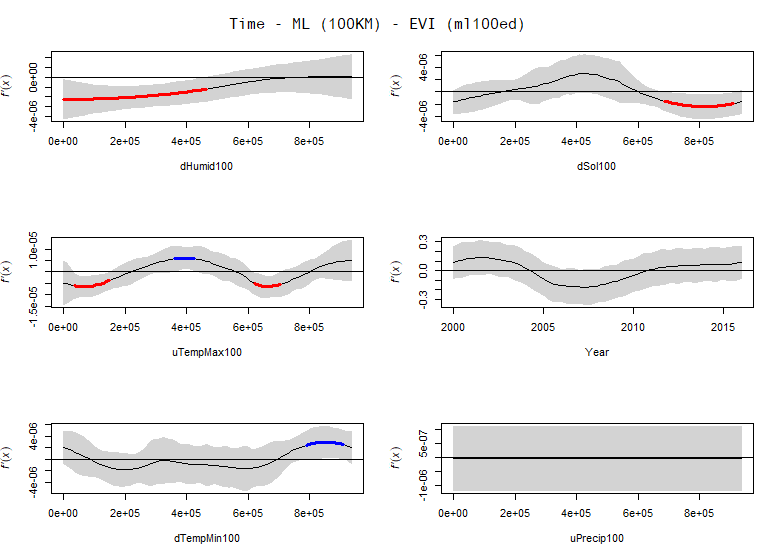
\includegraphics[width=1.2\textwidth]{ml100ed.png} % second figure itself
        \caption{\textbf{Model ml100ed}}
    \end{minipage}
\end{figure}


\begin{figure}[H]
  \centering
  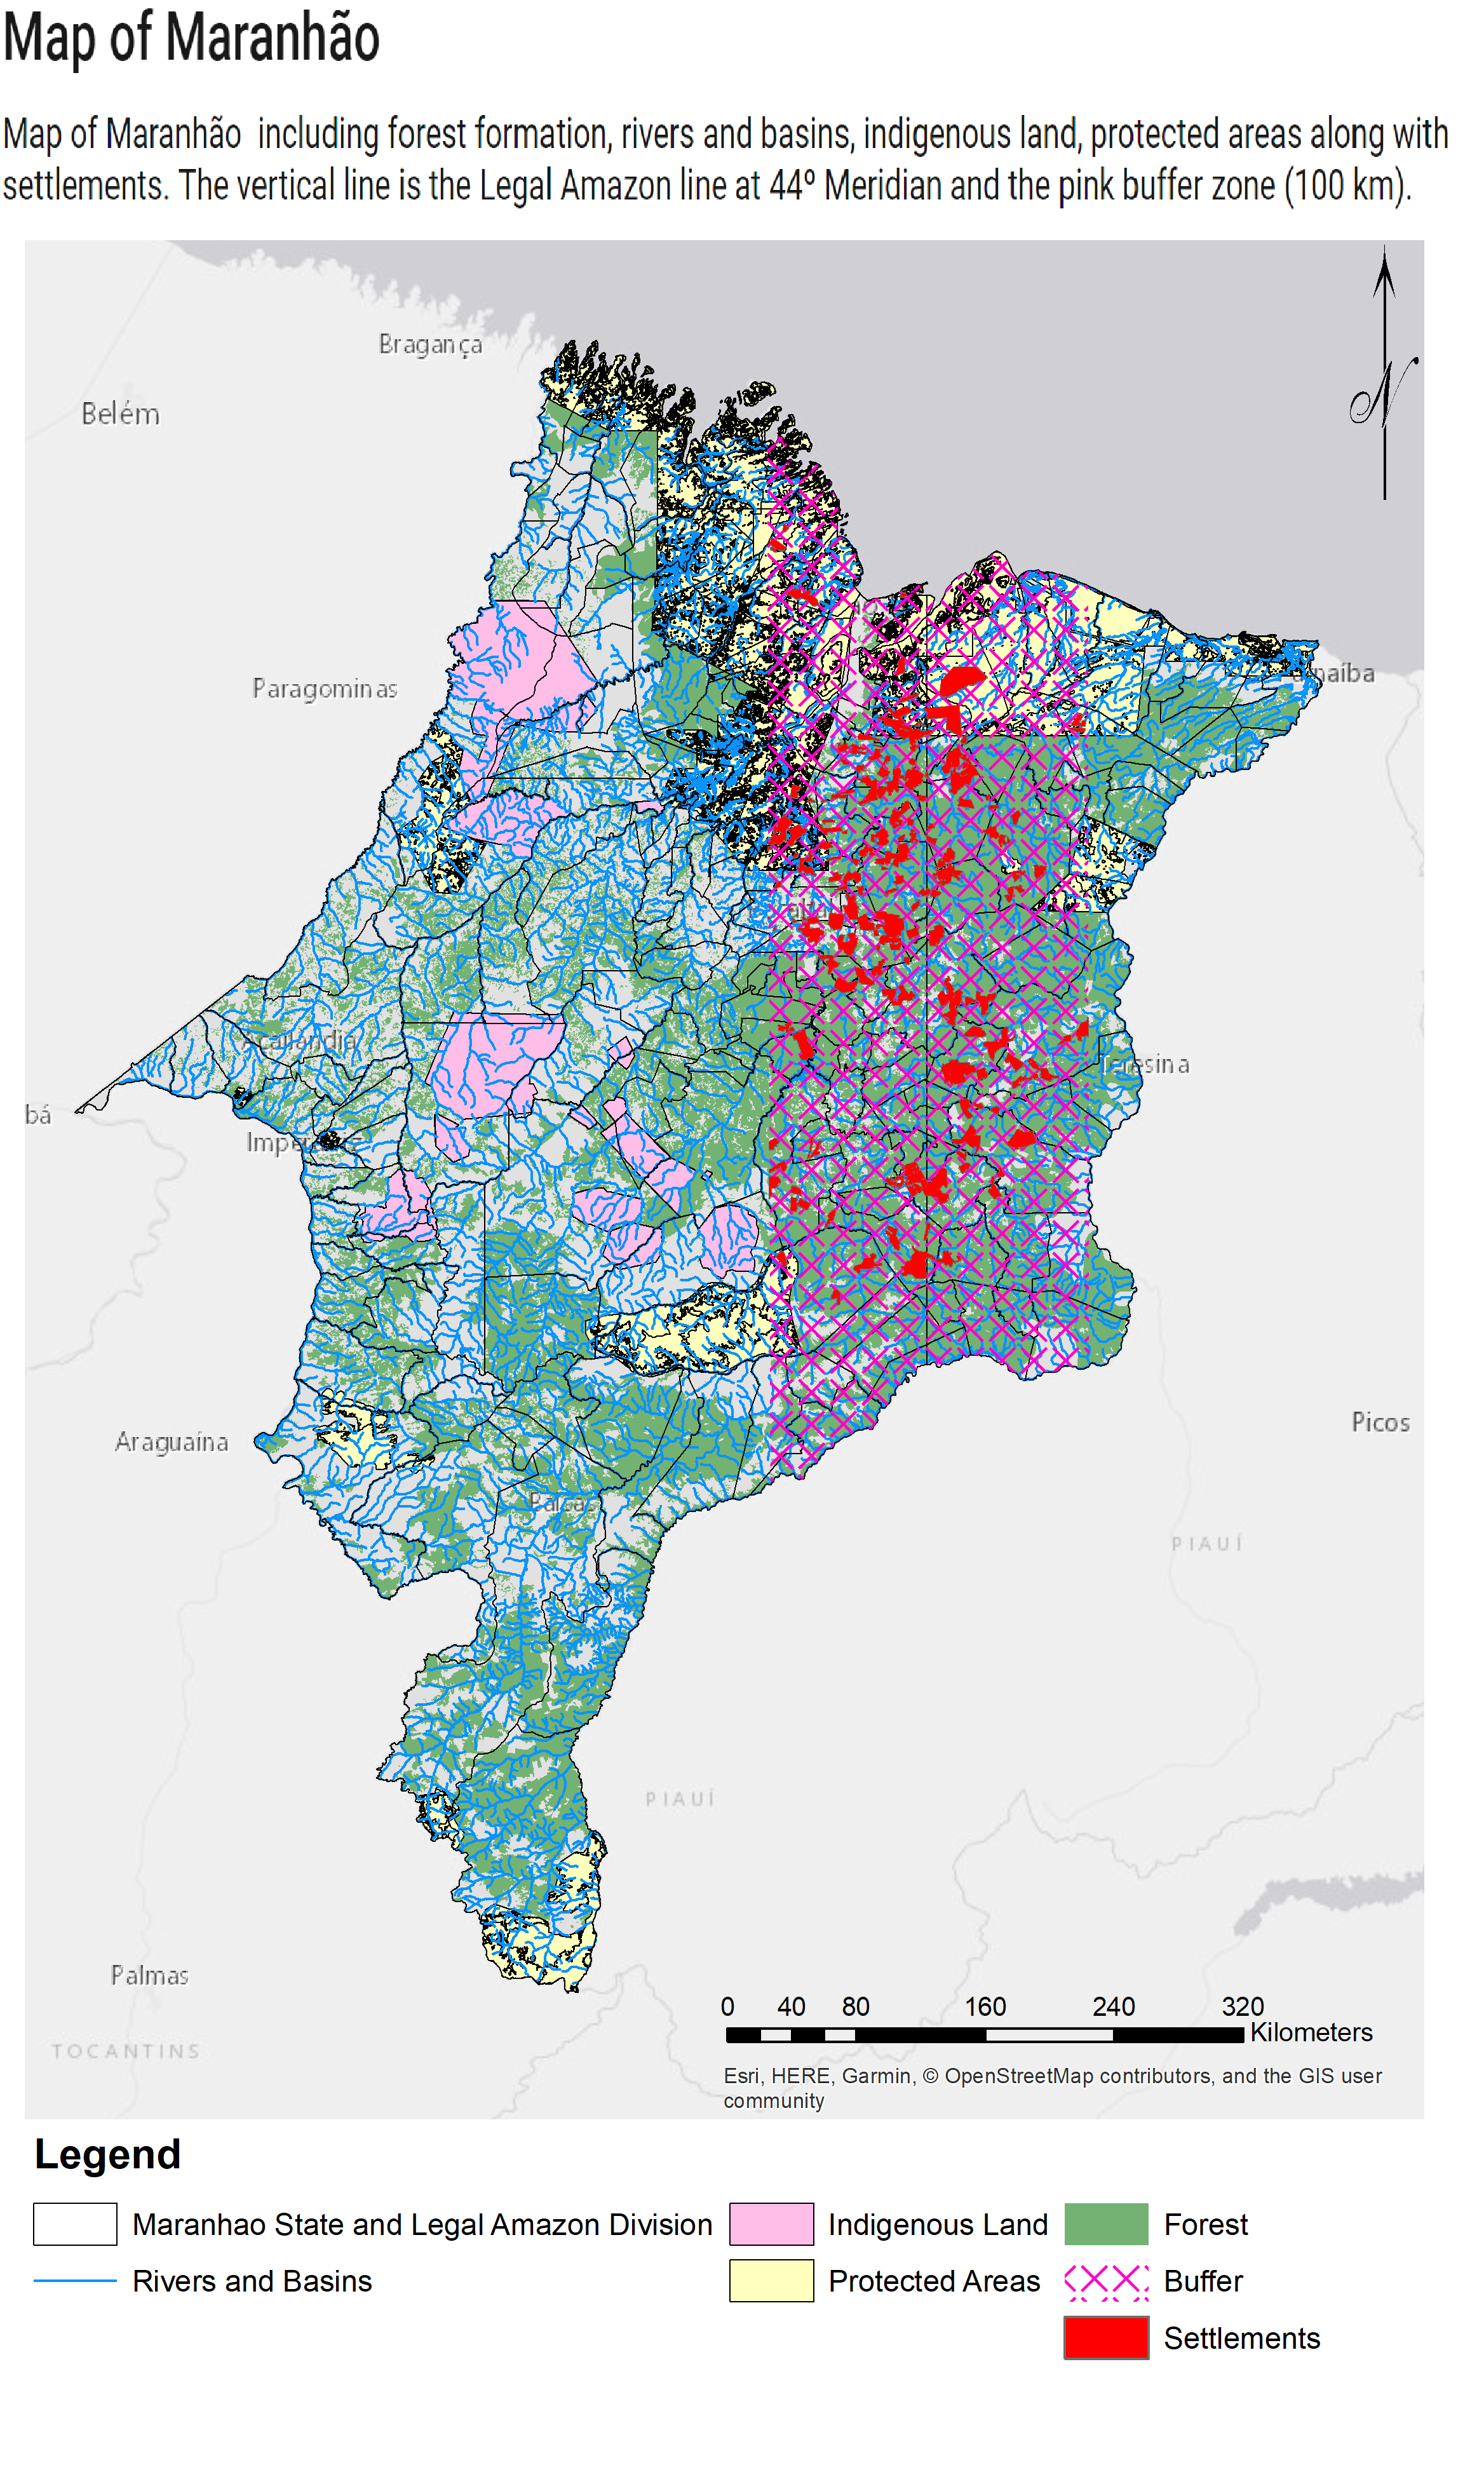
\includegraphics[width=0.9\textwidth, inner]{Settlements_title.png}
\caption{Source: \citep{MMMAwebsite,nugeo_2018,embrapa_2018, INCRA}.}
\label{fig:delimitacaosett}
\end{figure}



